\documentclass[
    10pt,
    % aspectratio=219,
    aspectratio=169,
    % aspectratio=11,
    % xcolor={dvipsnames},
    % hyperref={colorlinks=true,linkcolor=blue,urlcolor=blue}
]{beamer}

\renewcommand{\familydefault}{\rmdefault}

\usetheme{metropolis}

\usepackage{graphicx}
\usepackage{amsmath}
\usepackage{amssymb}
\usepackage{soul}
\usepackage{dirtree}
\usepackage{multicol}
\usepackage{hyperref}
\usepackage{cite}
\usepackage{listings}
\usepackage{pgfgantt}
\usepackage{xcolor}
\usepackage{tikz}


\definecolor{codegreen}{rgb}{0,0.6,0}
\definecolor{codegray}{rgb}{0.5,0.5,0.5}
\definecolor{codepurple}{rgb}{0.58,0,0.82}
\definecolor{backcolour}{rgb}{0.95,0.95,0.92}


\lstdefinestyle{mystyle}{
    backgroundcolor=\color{backcolour},   
    commentstyle=\color{orange},
    keywordstyle=\color{red},
    numberstyle=\tiny\color{codegray},
    stringstyle=\color{violet},
    basicstyle=\small\ttfamily,
    breakatwhitespace=false,         
    breaklines=true,                 
    captionpos=b,             
    keepspaces=true,                 
    numbers=left,                    
    numbersep=5pt,                  
    showspaces=false,                
    showstringspaces=false,
    showtabs=false,                  
    tabsize=4
}

\lstset{style=mystyle}

\title{
    % Comparitive Analysis of
    Classical and Quantum Markov-Chain Monte Carlo Method}
% \subtitle{Optimizing for Tomorrow's Discoveries}
\author{Meesum Qazalbash, Safi Haider}
  
\date[\today] % (optional)
{\today}

\logo{
\includegraphics[height=1cm]{hu-logo.jpg}}


\begin{document}
\maketitle

\begin{frame}{Outline}
    \tableofcontents
\end{frame}

\section{Metropolis-Hasting Algorithm}
\begin{frame}{Introduction}
    \begin{itemize}
        \item A Markov Chain Monte Carlo (MCMC) method.
        \item Used for obtaining a sequence of random samples from a probability distribution for which direct sampling is difficult.
        \item Application: Bayesian statistics, physics, and computational biology.
    \end{itemize}
\end{frame}

\begin{frame}{Basic Principle}
    \begin{itemize}
        \item Construct a Markov chain that has the desired distribution as its equilibrium distribution.
        \item The state of the chain after a large number of steps is then used as a sample of the desired distribution.
    \end{itemize}
\end{frame}

\begin{frame}{Algorithm Steps}
    \begin{itemize}
        \item Start with an arbitrary point \(x_0\).
        \item For each step \(t\), propose a new point \(y\) based on a proposal distribution \(q(y|x_t)\).
        \item Compute acceptance probability: \(\alpha = \min\left(1, \frac{p(y)q(x_t|y)}{p(x_t)q(y|x_t)}\right)\), where \(p\) is the target distribution.
    \end{itemize}
\end{frame}

\section{Classical MCMC}
\begin{frame}{Introduction}
    \begin{itemize}
        \item Classical MCMC is a family of algorithms used for sampling from probability distributions.
        \item Aim: To generate a sample of states from a distribution in scenarios where direct sampling is infeasible.
    \end{itemize}
\end{frame}

\begin{frame}{Core Principle}
    \begin{itemize}
        \item Utilizes Markov chains to produce a sequence of samples.
        \item Each sample's probability only depends on the state of the previous sample (Markov property).
    \end{itemize}
\end{frame}

\begin{frame}{Algorithm Structure}
    \begin{itemize}
        \item Starts from an initial state.
        \item Moves through the state space based on transition probabilities.
        \item The chain eventually reaches a stationary distribution.
    \end{itemize}
\end{frame}

\section{Ising Model}
\begin{frame}{Introduction}
    \begin{itemize}
        \item A mathematical model of ferromagnetism in statistical mechanics.
        \item Consists of discrete variables representing magnetic dipole moments of atomic spins, which can be in one of two states (+1 or -1).
    \end{itemize}
\end{frame}

\begin{frame}{Mathematical Formulation}
    \begin{itemize}
        \item The energy of a configuration is given by,
              \[ E(\mathbf{s}) = - \sum_{i>j}J_{ij} s_i s_j - h \sum_i h_is_i \]
        \item Where \( s_i \) are the spin values, \( J_{ij} \) the interaction strength, \( h_i \) the external magnetic field.
    \end{itemize}
\end{frame}

\begin{frame}{Boltzmann Distribution}
    \begin{itemize}
        \item The probability of a configuration is given by,
              \[ \mu(\mathbf{s}) = \frac{1}{\mathcal{Z}} exp{\left(- \frac{E(\mathbf{s})}{T}\right)} \]
        \item Where, \( Z \) is the partition function and \( T \) is the temperature.
    \end{itemize}
\end{frame}

\begin{frame}{Sampling from Boltzmann Distribution}
    Output random n-bit strings \(\mathbf{s}\) such that \(\operatorname{Pr}(\mathbf{s})\approx\mu(\mathbf{s})\).
    \[\langle f(\mathbf{s})\rangle=\sum_{\mathbf{s}}\mu(\mathbf{s})f(\mathbf{s})\approx\frac{1}{\text{\# of samples}}\sum_{\text{samples }\mathbf{s}\sim\mu}f(\mathbf{s})\]
\end{frame}

\section{Quantum MCMC}
\begin{frame}{Quantum MCMC}
    \begin{itemize}
        \item A quantum algorithm for sampling from probability distributions.
        \item The algorithm is based on the Metropolis-Hastings algorithm.
    \end{itemize}

    \begin{figure}
        \centering
        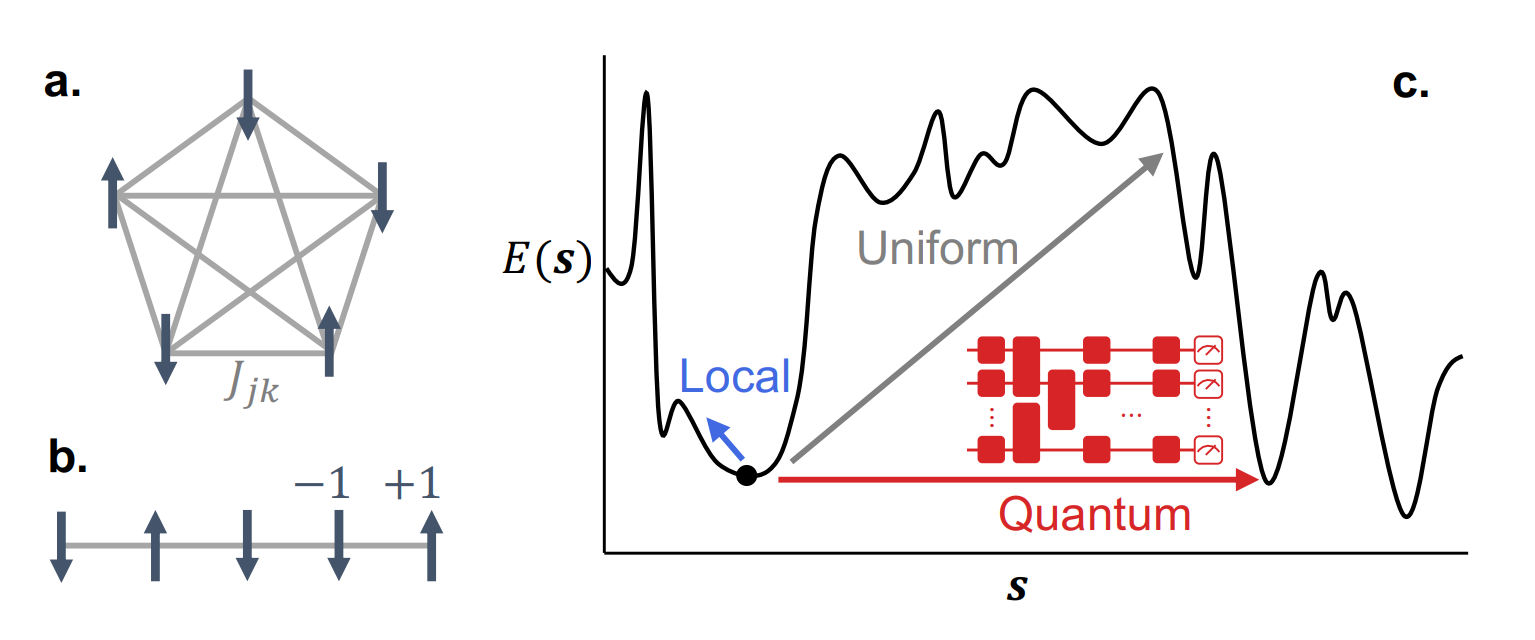
\includegraphics[width=0.8\textwidth]{1.png}
    \end{figure}
\end{frame}

\begin{frame}{Picking Transition Probabilities (Classical)}
    \textbf{Step 1}: Pick a transition probability \(T(\mathbf{s}\rightarrow\mathbf{s'})\).
    \[\text{Current state }\mathbf{s}\longrightarrow\text{Some mechanism}\longrightarrow\text{Proposed state }\mathbf{s'}\]
    \textbf{Step 2}: Ensure convergence, by computing,
    \[A=\min\left(1,\frac{\mu(\mathbf{s'})\operatorname{Pr}(\mathbf{s'}\rightarrow\mathbf{s})}{\mu(\mathbf{s})\operatorname{Pr}(\mathbf{s}\rightarrow\mathbf{s'})}\right)\]
    \textbf{Step 3}: Accept or reject the proposed state.
    \[\text{Accept }\mathbf{s'}\text{ with probability }A\text{, else stay at }\mathbf{s}\]
\end{frame}

\begin{frame}{Picking Transition Probabilities (Quantum)}
    \textbf{Step 1}:
    \begin{itemize}
        \item Prepare computational state \(\left|\mathbf{s}\right\rangle\).
        \item Evolve by \(H=\sum_{\mathbf{s}}\mu(\mathbf{s})\left|\mathbf{s}\right\rangle\left\langle\mathbf{s}\right|+\gamma T\).
        \item Measure in computational basis to get \(\mathbf{s'}\).
    \end{itemize}
    \textbf{Step 2}: Ensure convergence, by computing,
    \[A=\min\left(1,\exp{\left(-\frac{\Delta E}{T}\right)}\right)\]
    \textbf{Step 3}: Accept or reject the proposed state.
    \[\text{Accept }\mathbf{s'}\text{ with probability }A\text{, else stay at }\mathbf{s}\]
\end{frame}

\begin{frame}{Algorithm}
    \begin{figure}
        \centering
        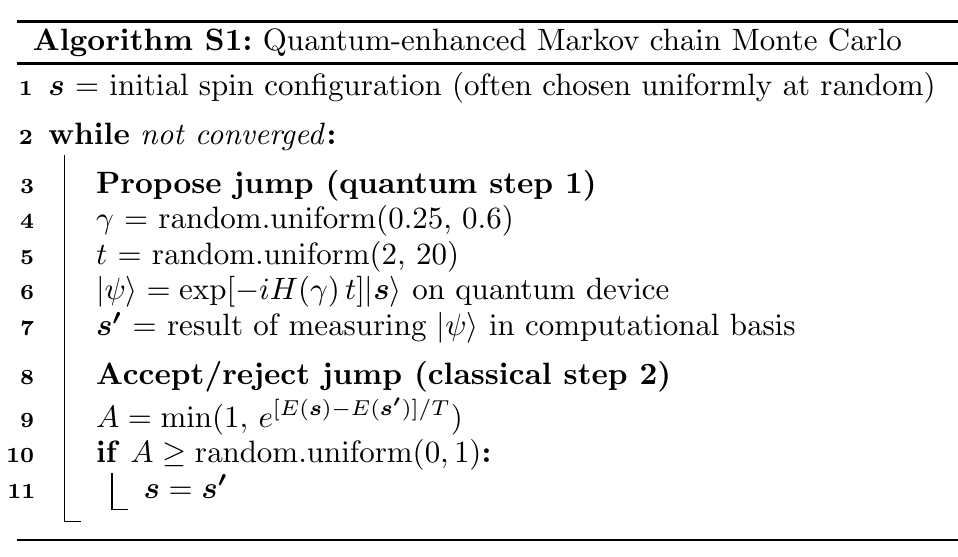
\includegraphics[width=0.8\textwidth]{4.png}
    \end{figure}
\end{frame}

\begin{frame}{Important Points}
    \begin{itemize}
        \item It is Semi-Heuristic; speed is established empirically.
        \item No variational optimization.
        \item Fails with increasing noise.
    \end{itemize}
\end{frame}


\section{Analysis}
\begin{frame}{Analysis}
    \begin{figure}
        \centering
        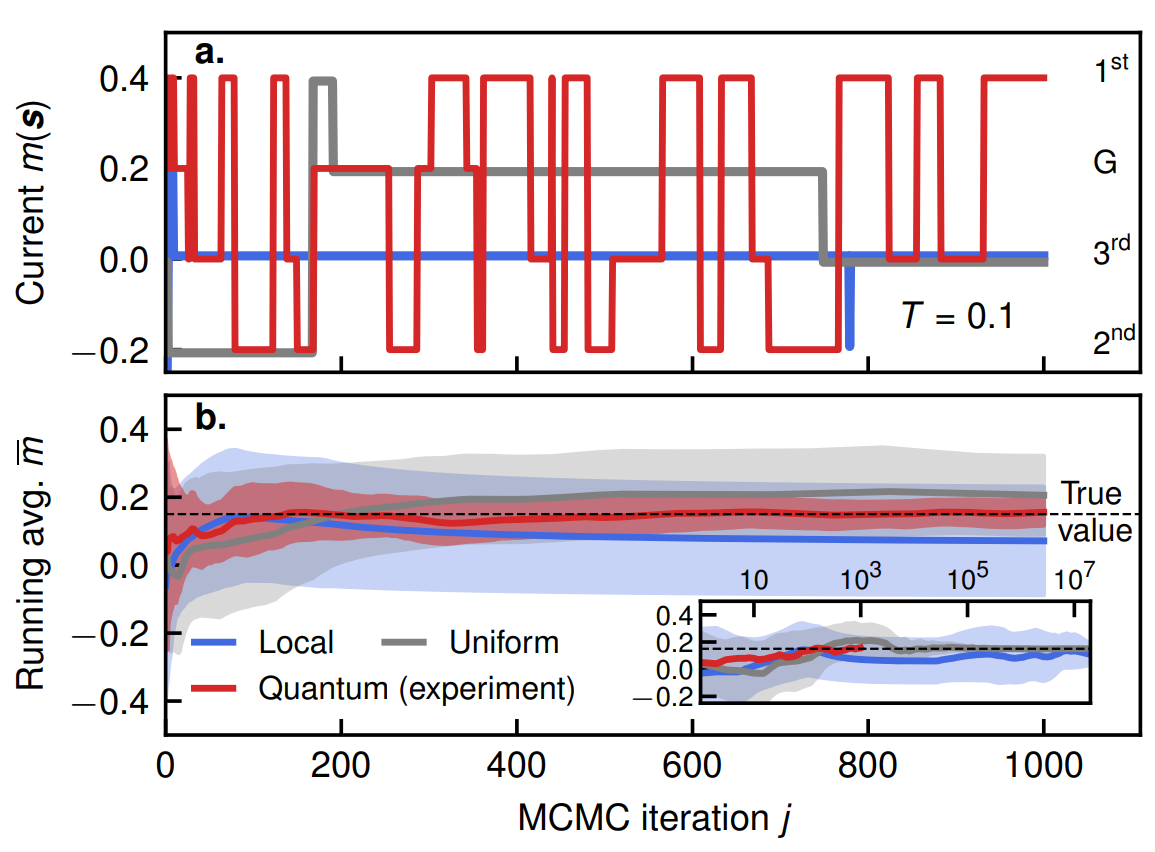
\includegraphics[width=0.6\textwidth]{2.png}
    \end{figure}
\end{frame}

\begin{frame}{Theory Vs Experiment}
    \begin{figure}
        \centering
        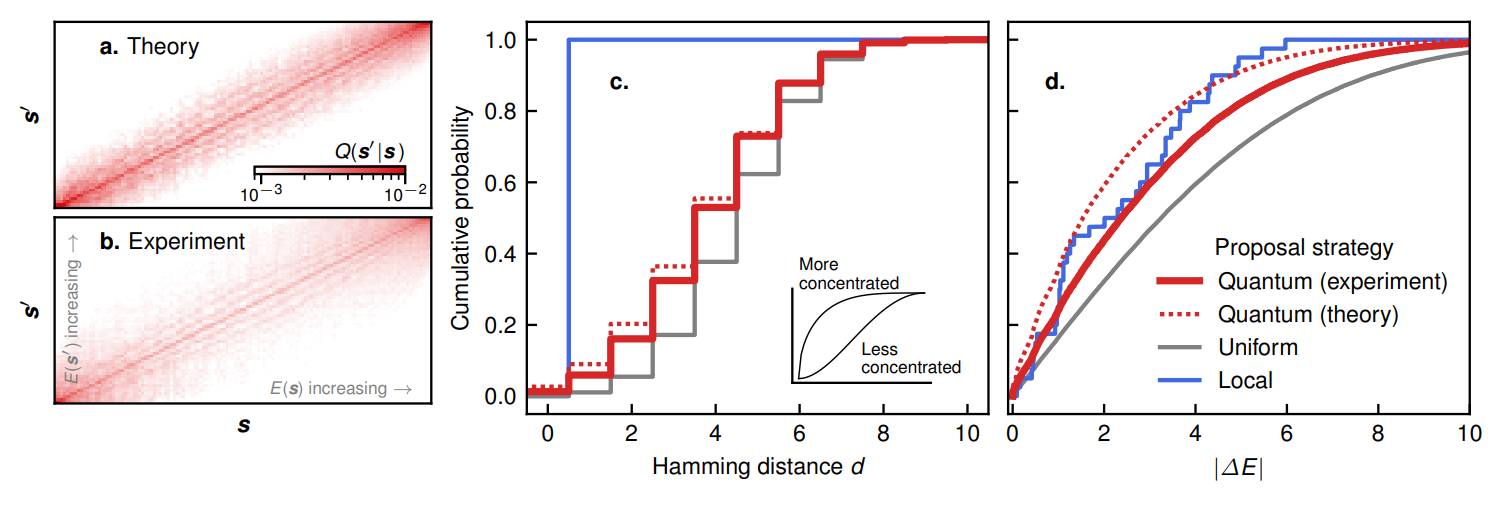
\includegraphics[width=0.8\textwidth]{3.png}
    \end{figure}
\end{frame}

\begin{frame}
    \begin{center}
        {\LARGE Questions?}
    \end{center}
\end{frame}

\end{document}